\section{Comparison with published FRB/US results}
\label{sec:comparison}

This section consolidates the paper's headline numbers against the published record in one place. Two kinds of comparison must be kept apart. The first is \emph{like-for-like}: the Fed's own \texttt{pyfrbus} reference implementation runs on this machine, on the same \texttt{model.xml}, the same LONGBASE vintage and the identical shock, so the two implementations should agree --- and they do, exactly. Re-running the Board's demo experiment (a 100-basis-point add-factor to \texttt{rffintay} under surplus-ratio fiscal targeting) in both codes gives a maximum absolute difference of $6.0\times10^{-9}$ across all 284 endogenous variables and all twenty quarters, i.e.\ solver-tolerance noise. The second kind of comparison is against \emph{published} FRB/US output --- most usefully the 2014 FEDS Note responses under VAR expectations \citep{brayton2014note} and the cross-model fiscal ranges of \citet{coenen2012effects} and \citet{whalen2015fiscal}. There the numbers can only be close, not identical: the published simulations were produced on earlier model and database vintages, from different baselines, and with shock designs (e.g.\ persistence of the funds-rate innovation) that the notes do not fully pin down. Table~\ref{tab:published-comparison} shows both kinds side by side.

\begin{table}[htbp]
\centering
\caption{This implementation versus the Fed's pyfrbus and published FRB/US results}
\label{tab:published-comparison}
\footnotesize
\begin{tabularx}{\textwidth}{>{\raggedright\arraybackslash}p{0.27\textwidth}l>{\raggedright\arraybackslash}X>{\raggedright\arraybackslash}X}
\toprule
Quantity & Ours & Published & Deviation and reading \\
\midrule
\multicolumn{4}{l}{\emph{100bp funds-rate shock (VAR expectations)}}\\
\quad Real GDP, trough & $-0.55\%$ (yr~2) & --- & FEDS Note reports the gap, not GDP \\
\quad Output gap, trough & $-0.50$pp (yr~1.5) & $\approx-0.4$pp max & $\approx0.1$pp deeper; vintage/shock design \citep{brayton2014note} \\
\quad Unemployment, peak & $+0.26$pp (yr~2) & rises (Okun-consistent) & consistent; peak $\approx$ half the gap trough \\
\quad Core PCE inflation, trough & $-0.034$pp (yr~2) & $\approx-0.08$pp & $0.05$pp smaller; flatter current-vintage Phillips curve \citep{brayton2014note} \\
\quad vs.\ vendor pyfrbus (like-for-like) & \multicolumn{2}{l}{identical to $6.0\times10^{-9}$ (284 vars)} & exact by construction \citep{fedfrbuspython} \\
\addlinespace
\multicolumn{4}{l}{\emph{Government purchases, 1\% of GDP}}\\
\quad Multiplier, yr~1, Taylor rule & $0.73$ & $0.7$--$1.0$ (no accommodation) & inside range \citep{coenen2012effects} \\
\quad Multiplier, yr~2, fixed funds rate & $0.99$ & ``roughly one'' pegged; $1.1$--$1.2$ with 2-yr accommodation & matches the Board's characterisation; just below cross-model accommodation range \citep{brayton2014note, coenen2012effects} \\
\addlinespace
\multicolumn{4}{l}{\emph{Personal tax cut, 1\% of GDP ex ante}}\\
\quad Multiplier, yrs~1--2 & $0.22\rightarrow0.32$ & $0.2$--$0.4$; CBO central $\approx0.3$ & inside both ranges \citep{coenen2012effects, whalen2015fiscal} \\
\bottomrule
\end{tabularx}

\medskip
\parbox{0.97\textwidth}{\footnotesize ``Ours'' entries are computed from \texttt{figures/results.json}. The pyfrbus row re-runs the Board's demo shock in the vendor package (relaxed dependency pins, Newton solver at \texttt{xtol}$=10^{-8}$) and in this implementation on the identical baseline. Published 100bp responses are read from the 2014 FEDS Note charts (VAR expectations) and are therefore approximate.}
\end{table}

The like-for-like agreement is the decisive test: on identical inputs the two codebases are the same model to solver precision, so the residual gaps against the 2014 FEDS Note --- a slightly deeper output-gap trough and a roughly half-as-large inflation response --- reflect model vintage and shock design, not implementation error. Both deltas move in the direction expected from documented vintage changes, most notably the progressive flattening of the estimated price Phillips curve between the 2014 public release and the current one. Figure~\ref{fig:cmp-multipliers} summarises the fiscal comparison graphically, Figure~\ref{fig:cmp-irf-feds} overlays the published peak responses on our impulse responses, and Figure~\ref{fig:cmp-pyfrbus} shows the ours-versus-pyfrbus overlay, in which the two lines are visually indistinguishable.

\begin{figure}[htbp]
\centering
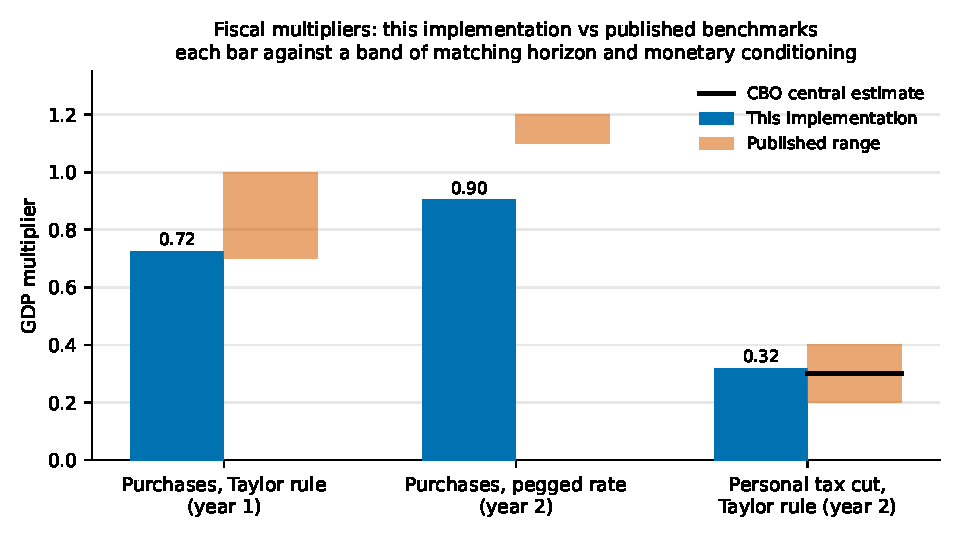
\includegraphics[width=0.85\textwidth]{figures/fig_cmp_multipliers.pdf}
\caption{Fiscal multipliers: this implementation (bars) against the \citet{coenen2012effects} cross-model ranges (bands) and the CBO central estimate \citep{whalen2015fiscal}.}
\label{fig:cmp-multipliers}
\end{figure}

\begin{figure}[htbp]
\centering
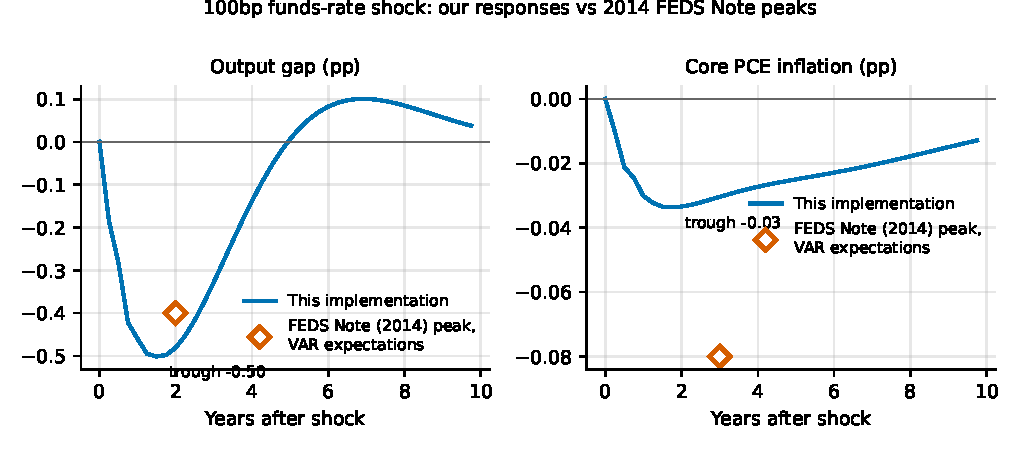
\includegraphics[width=0.95\textwidth]{figures/fig_cmp_irf_feds.pdf}
\caption{100bp funds-rate shock: our output-gap and core-inflation responses with the 2014 FEDS Note peak responses under VAR expectations \citep{brayton2014note} marked (diamonds; magnitudes read from the published charts, timing approximate).}
\label{fig:cmp-irf-feds}
\end{figure}

\begin{figure}[htbp]
\centering
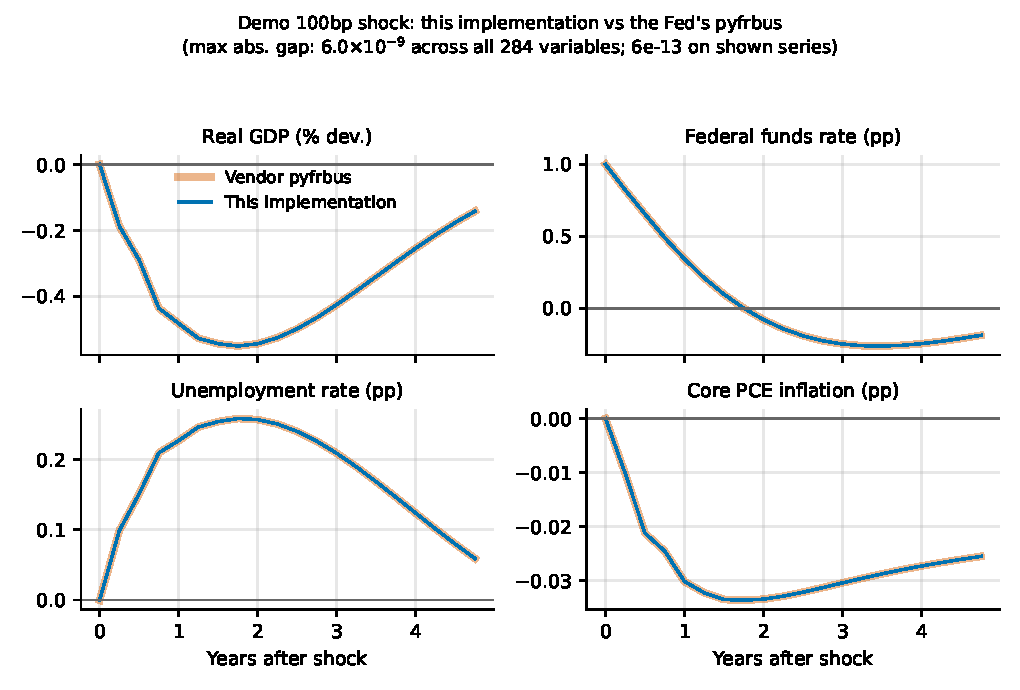
\includegraphics[width=0.9\textwidth]{figures/fig_cmp_pyfrbus.pdf}
\caption{Like-for-like validation: the Board's demo 100bp shock run in this implementation and in the vendor pyfrbus package. The thick and thin lines coincide; the maximum absolute gap is $6.0\times10^{-9}$ across all 284 endogenous variables ($6\times10^{-13}$ on the series shown).}
\label{fig:cmp-pyfrbus}
\end{figure}
